% !TEX TS-program = xelatex
% !TEX encoding = UTF-8
% !Mode:: "TeX:UTF-8"

\documentclass[onecolumn,oneside]{SUSTechHomework}

\usepackage{float}

\author{胡玉斌}
\sid{11712121}

\title{Lab 12}
\coursecode{CS315}
\coursename{Computer Security}

\begin{document}
  \maketitle

  \section*{Task 1:}
  Finding out the addresses of libc functions

  We can find that the address of \verb|system()| is \verb|0xb7da4da0| and that for \verb|exit()| is \verb|0xb7d989d0| 

  \begin{figure}[H]
    \centering
    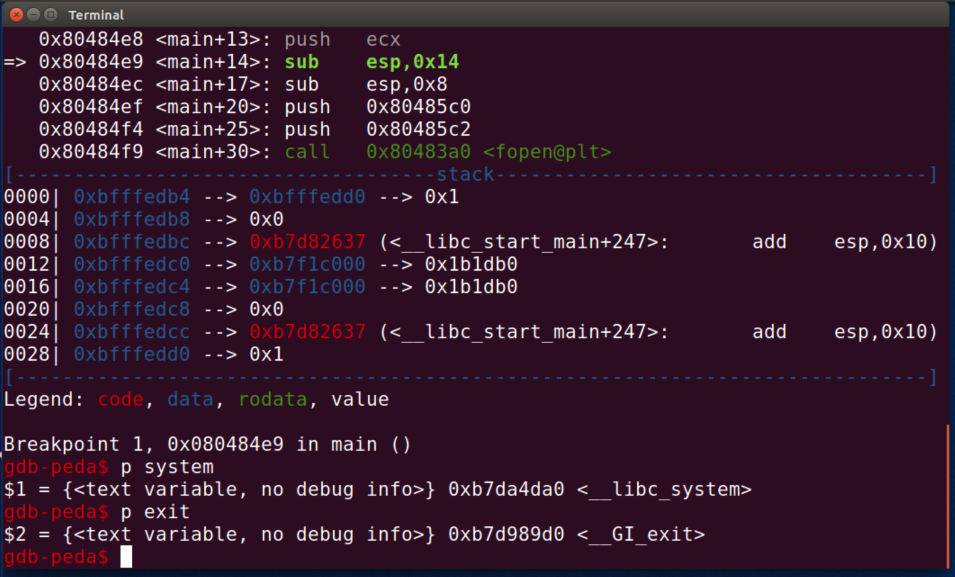
\includegraphics[width=0.85\textwidth]{img/task1_1.png}
    \caption{address of lib function}
  \end{figure}

  \section*{Task 2:}
  Putting the shell string in the memory

  Setting the config of bash environment, we can find the shell variable is \verb|0xbfffffec|

  \begin{figure}[H]
    \centering
    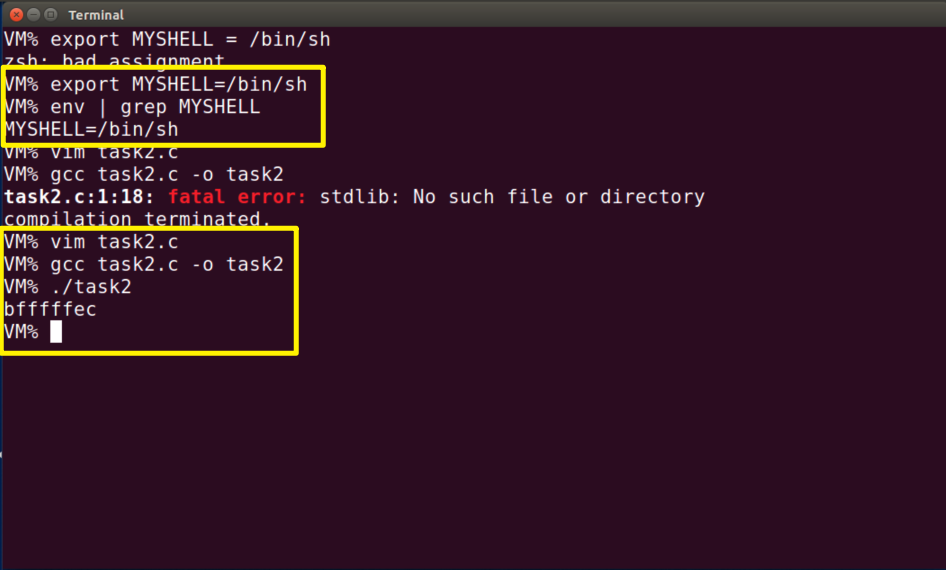
\includegraphics[width=0.85\textwidth]{img/task2_1.png}
    \caption{address of shell}
  \end{figure}

  \section*{Task 3:}
  Exploiting the Buffer-Overflow Vulnerability

  First, we generate the \verb|badfile|

  \begin{figure}[H]
    \centering
    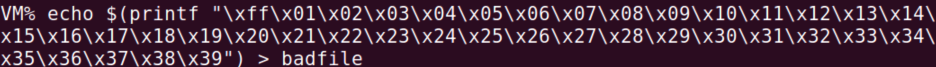
\includegraphics[width=0.85\textwidth]{img/task3_1.png}
    \caption{badfile}
  \end{figure}

  When we put the address which we find from task1 and task2 to the \verb|exploit.c|, we got error that it points to \verb|bin/sh|, so we modify \verb|0xbfffffec| to \verb|0xbfffffeb|

  \begin{figure}[H]
    \centering
    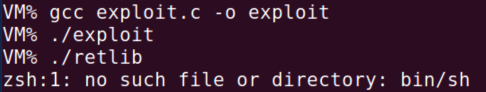
\includegraphics[width=0.85\textwidth]{img/task3_2.png}
    \caption{error address}
  \end{figure}

  success attack

  \begin{figure}[H]
    \centering
    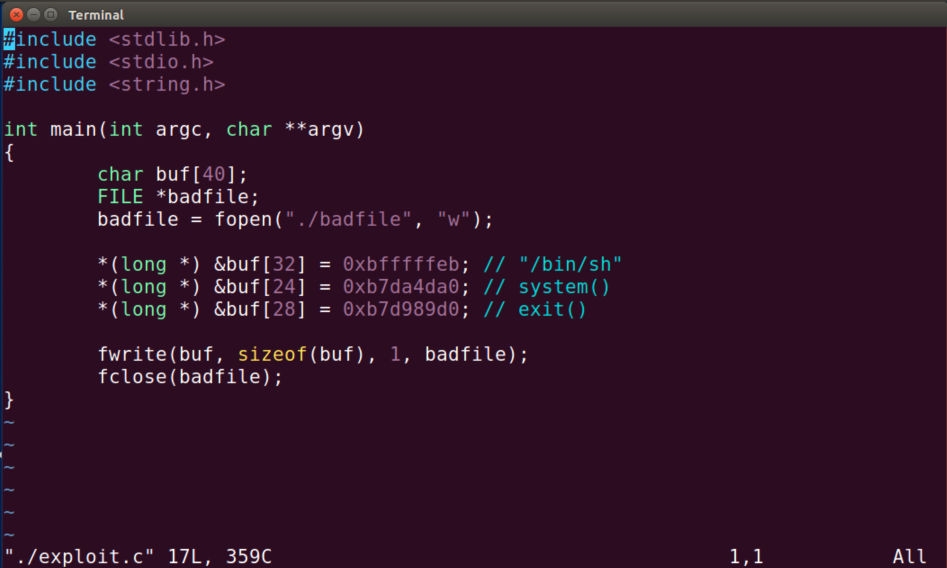
\includegraphics[width=0.85\textwidth]{img/task3_3.png}
    \caption{code}
  \end{figure}

  \begin{figure}[H]
    \centering
    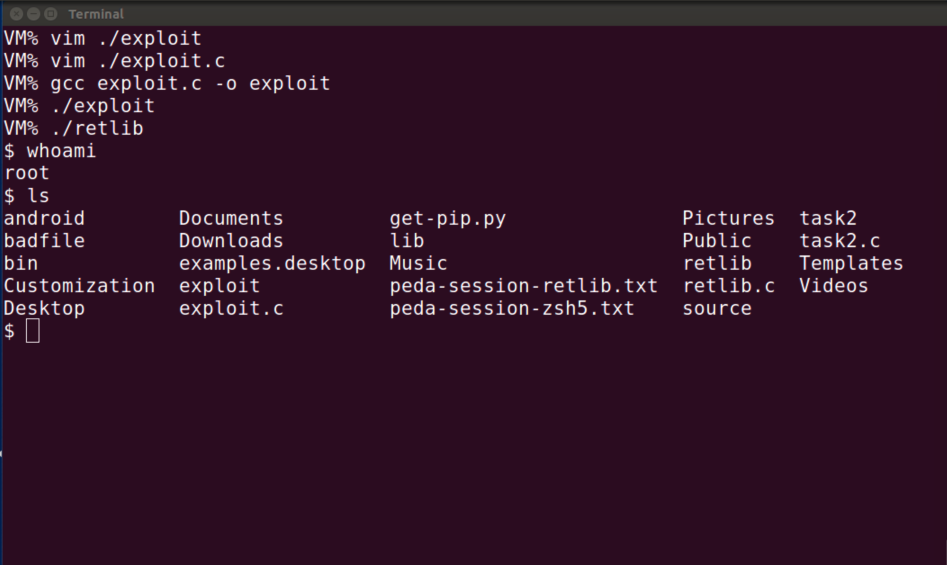
\includegraphics[width=0.85\textwidth]{img/task3_4.png}
    \caption{root shell}
  \end{figure}

  \subsection*{Attack variation 1:}

  Return address of \verb|system()| is not valid, so we will get \verb|segmentation fault|

  \begin{figure}[H]
    \centering
    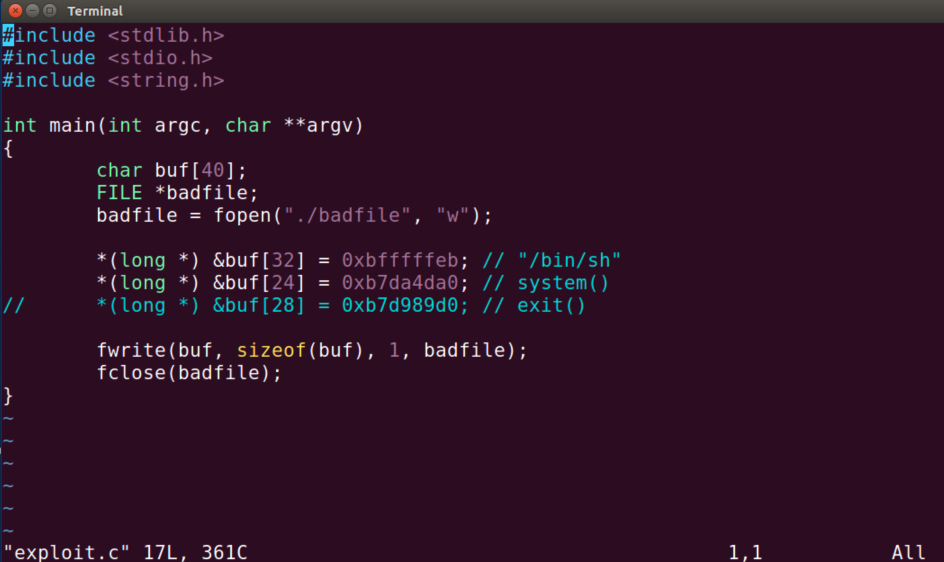
\includegraphics[width=0.85\textwidth]{img/task3_6.png}
    \caption{code}
  \end{figure}

  \begin{figure}[H]
    \centering
    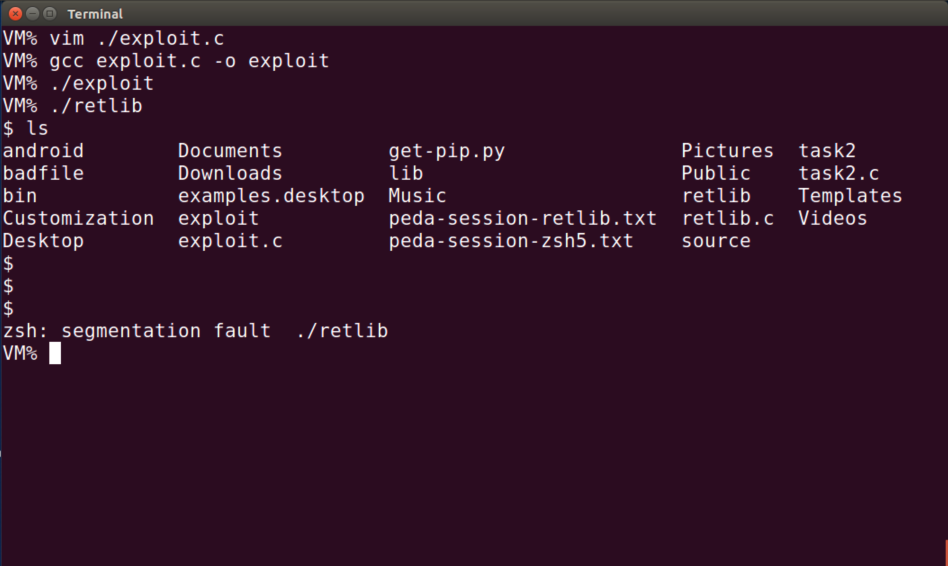
\includegraphics[width=0.85\textwidth]{img/task3_5.png}
    \caption{segmentation fault}
  \end{figure}

  \subsection*{Attack variation 2:}

  When we rename the \verb|retlib| to \verb|newreturn|, we cannot exploit successfully. The reason is that the address of \verb|MYSHELL| is changed with the name of the program is changed.

  \begin{figure}[H]
    \centering
    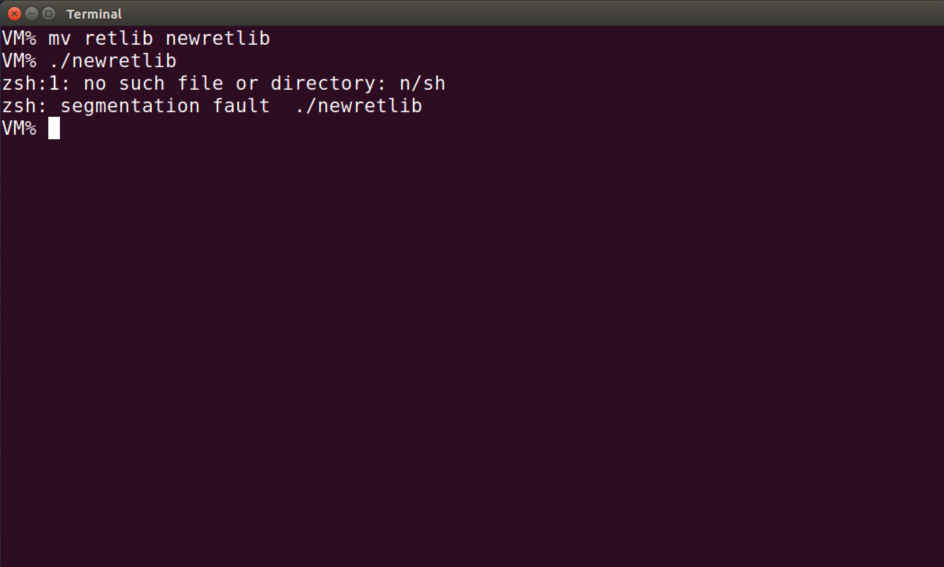
\includegraphics[width=0.85\textwidth]{img/task3_7.png}
    \caption{segmentation fault}
  \end{figure}

  \section*{Task 4:}
  Turning on Address Randomization

  We cannot exploit successfully when we turn on the randomization. And we got \verb|segmentation fault| when we repeat task1\&2.

  The address of \verb|MYSHELL| is changed randomly. \verb|system()| and \verb|exit()| are also changed.

  In \verb|exploit.c|, \verb|X, Y, Z| are correct, but \verb|buf[X], buf[Y], buf[Z]| are incorrect.
  
  \begin{figure}[H]
    \centering
    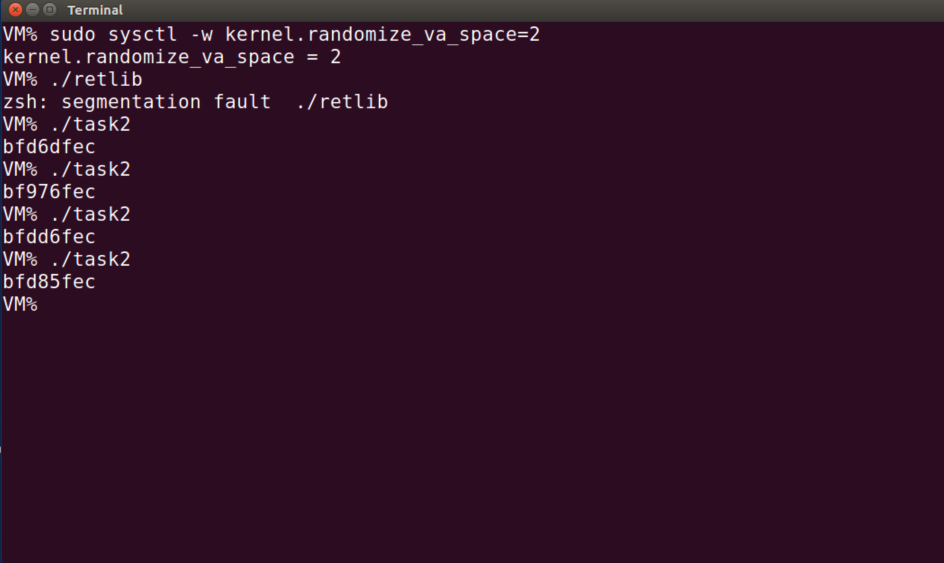
\includegraphics[width=0.85\textwidth]{img/task4_1.png}
  \end{figure}

  \begin{figure}[H]
    \centering
    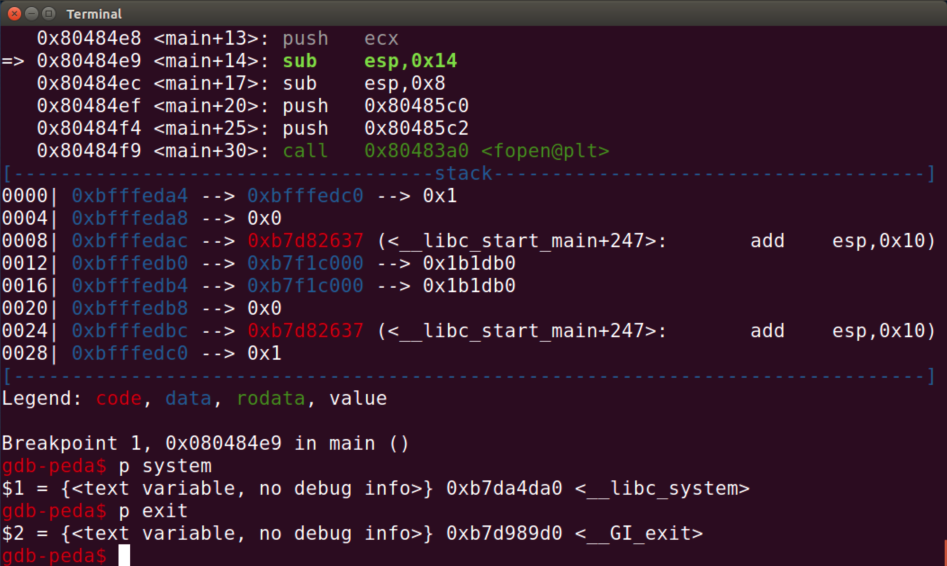
\includegraphics[width=0.85\textwidth]{img/task4_2.png}
  \end{figure}

\end{document}
